\section{Generality}
\label{sec:generality}

% as depicted in Figure~\ref{fig:workflow}
Although this paper examines the methodology on GPU Kepler architecture and shows its performance optimizations for SGEMM, we claim that the developed toolchain can be easily extended to other NVIDIA GPUs and the explored optimization strategies are applicable to other floating-point computation-intensive applications.

{\em {\bf Toolchain Portability}}: For a particular GPU architecture, users only need to regenerate disassembly codes from the PTX samples and microbenchmarks with CUDA binary utilities, and then feed them to the ISA encoding solver.
The opcode, modifier and operand solvers, are portable among GPU architectures. 
We have validated the solver functionalities on Fermi, Kepler, and Maxwell GPUs~\cite{artifact}. 
A corresponding assembler can be obtained by modifying the instruction grammar definition decoded by the solver, which could be automatically done with an assembler template~\cite{baldassin2005extending}.

{\em {\bf Optimizing CNN}}: The optimization strategies include
FFMA dual-issue, register allocation, memory load/store width, and instruction
scheduling. Note that the bare-metal tuning are more microarchitectural specific than application specific. With the support of a assemble language, our scheduling optimization is totally derived from instruction dependency and latency, which is not specific to SGEMM. With a proper blocking algorithm, multiple float computation instructions will be reside in a single loop iteration, then register allocation and dual issue optimization can refer SGEMM optimizations to improve floating-point computation throughput. 

Our convolution algorithm implementation uses $128\times128$ shared memory blocking and
$8\times8$ register blocking. We optimize it at assembly-level by using the method describe in section~\ref{sec:optimization}.
%The configuration of each layer can be found 
We benchmark three popular convolutional neural network:
Alexnet~\cite{krizhevsky2012imagenet}, Vgg~\cite{simonyan2014very} and
Overfeat~\cite{sermanet2013overfeat}.  The configuration of each convolutional
layer can be found in corresponding papers.
Figure~\ref{fig:conv} presents the performance of our optimized convolution and cuDNN by comparing the average performance of all the convolutional layers in a neural network. %The maximum convolution performance is 2653 Gflop/s.
Our optimized convolution implementations are 39\%, 46\% and 62\% higher than cuDNN V4.0 for the three CNN configurations respectively on Tesla K20m.

\begin{figure}[htbp]
\begin{center}
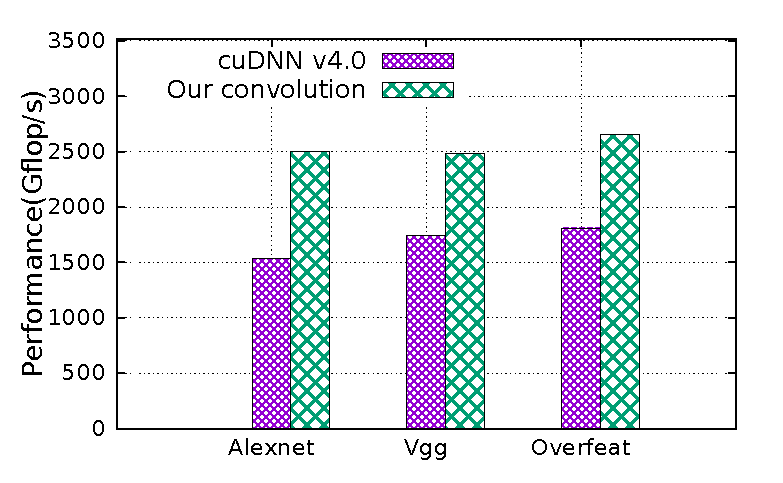
\includegraphics[scale=0.4]{cudnn}
    \caption{Performance comparison of cuDNN and our optimized convolution on GPU Tesla K20m (batch size is 128).}
\label{fig:conv}
\end{center}
\end{figure}
